% Created 2024-08-03 Sat 16:24
% Intended LaTeX compiler: pdflatex
\documentclass[10pt]{article}
% =================================BASE====================================%
\usepackage[left=2cm,right=2cm,top=2cm,bottom=2cm]{geometry} % Marges
\usepackage[T1]{fontenc} % Nécessaire avec FrenchBabel
\usepackage[utf8]{inputenc} % Important pour symboles Francophones, é,à,etc
\usepackage{csquotes} % Recommandé par PDFLatex lors de la compilation. 

% Calligraphie
%\usepackage{pxfonts} % Met le texte ET les maths en Palatino + donne accès à des symboles math
%\usepackage{palatino} % Cette commande met seulement le texte en police palatino
\usepackage{lmodern} % Pour les maths? Lmodern pour les maths
\usepackage{cfr-lm}
% Use lmodern for sans-serif
\usepackage{mathrsfs} % Permet la command \mathscr (Lettres attachées genre) \mathscr(B)

% Bibliographie
%\usepackage[backend=bibtex,style=phys,sorting=ynt]{biblatex}
\usepackage[backend=biber,sorting=ynt,style=authoryear]{biblatex} % N'est pas utilisé par le compilateur org-mode, mais NÉCESSAIRE. Voir le fichier init.el pour changer le style. 
\addbibresource{master-bibliography.bib}


\usepackage{amsmath, amssymb, amsthm} % Symb. math. (Mathmode+Textmode) + Beaux théorèmes.
\usepackage{mathtools,cancel,xfrac} % Utilisation de boîtes \boxed{} + \cancelto{}{}, xfrac
\usepackage{graphicx, wrapfig} % Géstion des figures.
\usepackage{hyperref} % Permettre l'utilisation d'hyperliens.
\usepackage{color} % Permettre l'utilisation des couleurs.
\usepackage{colortbl} % Color tables
\usepackage[dvipsnames]{xcolor} % Couleurs avancées.

% Physique
\usepackage{physics} % Meilleur package pour physicien. 

% Style
\usepackage{lipsum} % For fun
\usepackage{tikz} % Realisation de figures TIKZ.
\usetikzlibrary{arrows.meta,bending} % Arrow heads 
\usepackage{empheq} % Boite autour de MULTIPLE équations
\usepackage{bbding}

% Français
\usepackage[french]{babel} % Environnements en Français.

\usepackage{titling} % Donne accès à \theauthor, \thetitle, \thedate

% ==============================BASE-(END)=================================%





% ================================SETTINGS=================================%
% Pas d'indentation en début de paragraphe :
\setlength\parindent{0pt}
\setlength{\parskip}{0.15cm}

% Tableaux/tabular
% Espace vertical dans les tabular/tableaux
\renewcommand{\arraystretch}{1.2}
% Couleur des tableaux/tabular
% \rowcolors{3}{violet!5}{}

% Couleurs de hyperliens :
\definecolor{mypink}{RGB}{147, 0, 255}
\hypersetup{colorlinks, 
             filecolor=mypink,
             urlcolor=mypink, 
             citecolor=mypink, 
             linkcolor=mypink, 
             anchorcolor=mypink}


% Numéros d'équations suivent les sections :
\numberwithin{equation}{section} 

% Les « captions » sont en italique et largeur limitée
\usepackage[textfont = it]{caption} 
\captionsetup[wrapfigure]{margin=0.5cm}

% Retirer l'écriture en gras dans la table des matières
\usepackage{tocloft}
\renewcommand{\cftsecfont}{\normalfont}
\renewcommand{\cftsecpagefont}{\normalfont}

% Change bullet style
\usepackage{pifont}
\usepackage{enumitem}
%\setlist[itemize,1]{label=\ding{224}}
\setlist[itemize,1]{label=\ding{239}}
\renewcommand{\boxtimes}{\blacksquare}
% ================================SETTINGS=================================%



% ==============================NEWCOMMANDS================================%
% CQFD symbol
\renewcommand{\qedsymbol}{$\hfill\blacksquare$}

% Vecteurs de base :
\newcommand{\nvf}{\vb{\hat{n}}}
\newcommand{\evf}{\vb{\hat{e}}}
\newcommand{\ivf}{\vb{\hat{i}}}
\newcommand{\jvf}{\vb{\hat{j}}}
\newcommand{\kvf}{\vb{\hat{k}}}
\newcommand{\uu}{\vb{u}}
\newcommand{\vv}{\vb{v}}
\newcommand{\ust}{\vb{u}_{\ast}}

% Physics empty spaces 
\newcommand{\short}{\vphantom{pA}}
\newcommand{\tall}{\vphantom{pA^{x^x}_p}}
\newcommand{\grande}{\vphantom{\frac{1}{xx}}}
\newcommand{\venti}{\vphantom{\sum_x^x}}
\newcommand{\pt}{\hspace{1pt}} % One horizontal pt space

% Moyenne numérique entre deux points de grilles. 
\newcommand{\xmean}[1]{\overline{#1}^x}
\newcommand{\ymean}[1]{\overline{#1}^y}
\newcommand{\zmean}[1]{\overline{#1}^z}
\newcommand{\xymean}[1]{\overline{#1}^{xy}}

% Tilde over psi
\newcommand{\tpsi}{\tilde{\psi}}
\newcommand{\tphi}{\tilde{\phi}}

% Nota Bene env : (\ding{89})
%\newcommand{\nb}{$\boxed{\text{\footnotesize\EightStarConvex}\pt \mathfrak{N. B.}}$\hspace{4pt}}
\newcommand{\nb}{\underline{{\footnotesize\EightStarConvex}\pt $\mathfrak{N.B.}$\vphantom{p}}\hspace{3pt}}

\newcommand{\exemple}{
\parbox[center]{2.2cm}{\begin{tcolorbox}[sharp corners, rounded corners=northeast, rounded corners=southeast,
colback=Violet!2, colframe=black,
size=small, width=2cm, left=-0.25pt, bottom=-0.5pt,
arc is angular, arc=2.5mm, boxrule=0.35pt, leftrule=4pt, %bottomrule=1pt,
after={\enskip}] Exemple \end{tcolorbox}}}

\newcommand{\rad}{\text{Rad}}


\newcommand{\cqfd}{\hfill$\blacktriangleleft$}

% Define the nota bene environment
\usepackage{tcolorbox}
\newtcolorbox{notabene}{
     colback=blue!5,
     colframe=black,
     boxrule=0.5pt,
     arc=2pt,
     left=5pt,
     right=5pt,
     top=5pt,
     bottom=5pt,
}


\newcommand{\cmark}{\ding{52}}
\newcommand{\xmark}{\ding{55}}
% ==============================NEWCOMMANDS================================%



% ==============================PAGE-TITRE=================================%
% Titlepage 
\newcommand{\mytitlepage}{
\begin{titlepage}
\begin{center}
{\Huge \thesubtitle \par}
\vspace{2cm}
{\Huge \MakeUppercase{\thetitle} \par}
\vspace{2cm}
RÉALISÉ DANS LE CADRE\\ D'UN PROJET POUR \par
\vspace{2cm}
{\Huge ISMER--UQAR \par}
\vspace{2cm}
{\thedate}
\end{center}
\vfill
Rédaction \\
{\theauthor}\\
\url{charles-edouard.lizotte@uqar.ca}\\
ISMER-UQAR\\
Police d'écriture : \textbf{CMU Serif Roman}
\end{titlepage}
}
% ==============================PAGE-TITRE=================================%



% =================================ENTÊTE==================================%
\usepackage{fancyhdr}
\pagestyle{fancy}
\setlength{\headheight}{13pt}
\renewcommand{\headrulewidth}{0.025pt} % Ligne horizontale en haut

\fancyhead[R]{\textit{\thetitle}}
\fancyhead[L]{\ \thepage}
\fancyfoot[R]{\textit{\theauthor}}
\fancyfoot[L]{}
\fancyfoot[C]{} 
% =================================ENTÊTE==================================%
\author{Charles-Édouard Lizotte}
\date{28/07/2023}
\title{Carnet de bord, Université McGill}
\newcommand{\thesubtitle}{Contrat Été 2023}
\hypersetup{
 pdfauthor={Charles-Édouard Lizotte},
 pdftitle={Carnet de bord, Université McGill},
 pdfkeywords={},
 pdfsubject={},
 pdfcreator={Emacs 29.4 (Org mode 9.7.8)}, 
 pdflang={French}}
\begin{document}

\mytitlepage
\tableofcontents\newpage
\section{Mettre à jour portable pour travail à distance  \textit{<2023-07-24 Mon>}}
\label{sec:org0da0b24}

De manière générale, j'utilise l'ordinateur de bureau fourni par l'université McGill pour travailler.
Tout ça me permet d'avoir un meilleurs service sur l'installation des module (\emph{packages}).
La proximité de Ambrish, soit le James Caveen de McGill, m'aide beaucoup à comprendre comment tout ça fonctionne.
Cependant, je n'ai pas pris le temps de mettre cet ordinateur portable à jour.
Aujourd'hui est donc une bonne occasion de le faire.
\begin{itemize}
\item[{$\boxtimes$}] Cloner le \emph{.emacs.d} ;
\item[{$\boxtimes$}] Mise à jour de tous les modules MELPA pour Emacs ;
\item[{$\boxtimes$}] Installer les packages \LaTeX{}.
\item[{$\boxtimes$}] Cloner la dossier Documentation et tous les rapports ;
\item[{$\boxtimes$}] Cloner la branche \emph{walls} du modèle \emph{shallow water} ;
\end{itemize}
\section{Retour sur les conditions frontières \textit{<2023-07-26 Wed>}}
\label{sec:org620499c}

\begin{wrapfigure}[20]{r}{0.45\textwidth}
\vspace{-\baselineskip}
\begin{center}
\begin{tikzpicture}
%
\foreach \i in {0,1,2,3}
{\foreach \j in {-1,0,1,2,3}
{\draw [thick, red!40] (\i,\j+1) -- (\i,\j) ;
 \draw [thick,blue!40] (\j,\i) -- (\j+1,\i) ;}}
%
\foreach \i in {0,1,2,3}
{\foreach \j in {-1,0,1,2,3}
{\draw [-latex,thin,red!40 ] (\i,0.5+\j) -- (\i+0.15,0.5+\j);
 \draw [-latex,thin,blue!40] (0.5+\j,\i) -- (0.5+\j,\i+0.15);}}
% Domaine (Rectangle autour)
\draw [dotted] (0,0) rectangle (3,3);
% Cercles (Centres) :
\foreach \i in {0,1,2,3,4}
{\foreach \j in {0,1,2,3,4}
{\fill[fill=black ] (\i-0.5,\j-0.5) circle (0.9pt);}}
% Rectangles (Noeuds) :
\foreach \i in {0,1,2,3}
\foreach \j in {0,1,2,3}
{{\filldraw [black!85] (\i-0.03,\j-0.03) rectangle (\i+0.03,\j+0.03);}}
% Rulers 
\draw[> = latex, arrows = {|<->|}, thin,red ] (0,4.5) -- (3,4.5);
\draw (1.5,4.5) node [above,red] {nx};
\draw[> = latex, arrows = {|<->|}, thin,blue] (-1.5,0) -- (-1.5,3);
\draw (-1.5,1.5) node [above,blue,rotate=90] {ny};
\draw[> = latex, arrows = {|<->|}, thin,black!50] (4.5,-1) -- (4.5,4);
\draw (4.5,1.5) node [below,black!50,rotate=90] {$[0:\text{ny}+1]$};
\draw[> = latex, arrows = {|<->|}, thin,black ] (-0.5,-1.5) -- (3.5,-1.5);
\draw (1.5,-1.5) node [below,black] {$[0,\text{nx}]$};
%
\draw (0.5,-0.15) node [] {\color{blue}\tiny$v\pt(1,1)$};
\draw (-0.15,0.5) node [rotate=90] {\color{red}\tiny$u\pt(1,1)$};
% Ghost points (mailles):
\draw [black!20] (-1,-1) rectangle (4,4);
\foreach \i in {0,1,2,3,4}
{
\draw [-latex,thin,black!20] (-1,-0.5+\i) -- (-0.85,-0.5+\i);
\draw [-latex,thin,black!20] (4.0,-0.5+\i) -- (4.15,-0.5+\i);
\draw [-latex,thin,black!20] (-0.5+\i,-1) -- (-0.5+\i,-0.85);
\draw [-latex,thin,black!20] (-0.5+\i,4) -- (-0.5+\i,4.15);
}
% Ghost points (noeuds) :
\foreach \i in {-1,0,1,2,3,4}
{
\filldraw [black!20] (-1-0.03,\i-0.03) rectangle (-1+0.03,\i+0.03);
\filldraw [black!20] (4-0.03,\i-0.03) rectangle (4+0.03,\i+0.03);
\filldraw [black!20] (\i-0.03,-1-0.03) rectangle (\i+0.03,-1+0.03);
\filldraw [black!20] (\i-0.03,4-0.03) rectangle (\i+0.03,4+0.03);
};
% Ghost text : 
\draw (-0.5,-1.15) node [gray] {\tiny$v\pt(0,0)$};
\draw (-1.15,-0.5) node [gray,rotate=90] {\tiny$u\pt(0,0)$};
\end{tikzpicture}
\end{center}
\caption{\label{orgaebfb4e}Exemple de grille avec frontières fixes (nx\pt=\pt ny\pt=\pt4). Pointillé central définit les frontière «\pt réelles\pt» du modèle tandis que tous les points aux alentours sont des points fantômes.}
\end{wrapfigure}

Au \href{rapport-2023-07-07.org}{dernier rapport}, nous avons posé les bases d'un modèle emboîté par de frontières de conditions \emph{no normal flow} et \emph{free slip}.
Autrement dit, aucun courant ne traverse les frontières et la contrainte de cisaillement normales à ces dernières est nulle. \bigskip

Tout juste avant les vacances \footnote{Rencontre effectuée le 14 juillet 2023}, David et Louis-Philippe avaient fortement insisté sur la nécessité de garder tous points de grille fantôme provenant de l'ancien modèle.
Principalement, le but de l'exercice est de voir si des erreurs se glissent entre les lignes de notre code. \bigskip

Un bref résumé des sous-routines à modifier en terme de mailles : 
\begin{itemize}
\item[{$\square$}] \emph{main.f90}
\item[{$\boxtimes$}] \emph{rhs.f90}
\item[{$\boxtimes$}] \emph{p correction.f90}
\item[{$\boxtimes$}] \emph{diags.f90}
\item[{$\boxtimes$}] \emph{init mudpack.f90}
\item[{$\boxtimes$}] \emph{div vort.f90}
\item[{$\boxtimes$}] \emph{divBT.f90}
\end{itemize}
\subsection{Tailles des quantités}
\label{sec:org32b20fc}
Principalement, on peut diviser nos quantités physiques en trois catégories, soient les \textbf{mailles} (\(\rightarrow\)), les \textbf{noeuds} (\(\blacksquare\)) et les \textbf{centres} (\(\bullet\)).
Chacune des quantités physique devra avoir une taille préférentielle.
Bien qu'on me l'aille déconseillé, je tiens à quand même « tenir mon bout » pour qu'on change les tailles de domaine un peu partout.
La raison me motivant est extrêmement simple : nous verrons bien plus facilement les erreurs fatales si ce sont des erreurs de code plutôt que des erreurs mathématiques.
On essaie tout ça aujourd'hui, si ça marche pas, on passe définitivement à autre chose.
\subsubsection{Les mailles (\(\rightarrow\))}
\label{sec:org1b58cf4}
Les mailles font référence aux vitesses et au \emph{RHS} de ces dernières. 
Dans la figure \ref{orgaebfb4e}, ces quantités sont illustrées à l'aide des couleurs bleu et rouge.
\begin{verbatim}
  real :: u(0:nx+1,0:ny), v(0:nx,0:ny+1)
\end{verbatim}
Ces quantités ont des tailles non-homogènes, car elles n'ont pas les mêmes orientations.
\subsubsection{Les centres (\(\bullet\))}
\label{sec:org23ba30d}
Les centre font référence aux quantités physiques qui se retrouvent au milieu des carrés dans une grille Arakawa-C.
On fait donc référence à la variation de l'interface \(\eta\), à la divergence, etc.
\begin{verbatim}
  real :: eta(0:nx,0:ny)
  real :: div(0:nx,0:ny)
\end{verbatim}
\subsubsection{Les noeuds (\(\blacksquare\))}
\label{sec:orgcf8ef55}
Les noeuds font déférence à quantités physiques aux jonctions entre les courants, donc les coins de nos carrés.
Ces quantités sont généralement reliées à un rotationnel, tel que la fonction de courant \(\psi\), la vorticité \(\zeta\) et la fréquence de Coriolis \(f\).
\begin{verbatim}
  real :: psi(0:nx+1,0:ny+1)
  real :: zeta(0:nx+1,0:ny+1)
\end{verbatim}
\subsection{Mention spéciale pour les boucles (do loop)}
\label{sec:org47169f4}

Puisque les conditions frontières \emph{no normal flow} et \emph{free slip} contraignent le système à avoir des courants nuls ou répétitifs, on se permet d'itérer entre \(i=2,\pt nx-1\).
Par la suite, on applique ces mêmes conditions frontière pour pallier les points qui n'ont pas été itérés.
D'un côté, ça nous sauve du temps de calcul et de l'autre, ça nous permet de seulement itérer sur ce qu'on a besoin d'itérer.\bigskip

Pour n'en nommer que quelques unes,
\begin{itemize}
\item Les \textbf{mailles} (\emph{edges}) n'ont besoin que d'être mises à jour qu'entre i,\pt j = 1 à nx,\pt ny-1.
C'est nécessaire si l'on veut veut faire nos applications sur tous les courants.
\item Les \textbf{noeuds} (/nodes) sont mis à jours entre i,\pt j = 2 à nx,\pt ny-1, car les fonctions de courants (\(\psi\)) et les vorticitées (\(\zeta\)) sont nulles aux frontières.
\item Les \textbf{centres} sont mis à jour de 1 à nx,\pt ny-1, car le reste est constitué de points fantômes.
\end{itemize}
\subsection{Expansion en série de Taylor pour le Laplacien}
\label{sec:org0ea9841}
Précédemment, nous avions développé l'expression de la dérivée seconde pour les murs.
Nous allons réaliser un petit rappel, car ça «\pt fait un boutte\pt» que je l'ai réalisé.
Sans oublier que j'ai besoin d'une référence accessible juste ici.\bigskip

On réalise deux expansions en série de Taylor depuis le mur pour les premiers et seconds points.
Ainsi
\begin{align}
   &&\boxed{\text{A}} && &u(2) = \cancelto{0}{u(1)} + \Delta x \cdot u'(1) + \qty(\frac{\Delta x^2}{2}) \ u''(1) && &&\\
   &&\boxed{\text{B}} && &u(3) = \cancelto{0}{u(1)} + 2\Delta x \cdot u'(1) + \qty(\frac{4\pt \Delta x^2}{2}) \ u''(1) && &&
\end{align}
Par la suite, on soustrait les équations de sorte à éliminer la dérivée première du courant, soit \(B - 2A\),
\begin{equation}
   u(3) - u(2) = 2\pt \Delta x^2 u''(1) - \Delta x^2 u''(1).
\end{equation}
Au final,
\begin{equation}
   \boxed{\hspace{0.3cm} u''(1) = \frac{u(3)-u(2)}{\Delta x^2}.\hspace{0.3cm}}
\end{equation}
Très simple.
\section{Gros ménage du modèle numérique \textit{<2023-07-28 Fri>}}
\label{sec:orged19e16}

\subsection{Purge des modules et sous-routines FFT dans la branche «\pt walls\pt»}
\label{sec:org714bd6a}
Étant donné que notre modèle ne fonctionnera uniquement qu'avec la suite MUDPACK, on se permet de purger tout ce qui est relié aux transformées de Fourier.
Deux raisons motivent cette actions  : 
\begin{enumerate}
\item Principalement, la plupart des quantités et sous-routines qui y sont reliés servent à faire des diagnostiques, donc je crois qu'on peut les retirer sans problème.
Mentionnons aussi que ces sous-routines ne fonctionneront tout simplement plus, considérant que notre domaine ne sera pas périodique.
\item En second plan, toutes les sous-routines et quantités retirées existent séparément sur mon \href{https://github.com/charli1213/Modele-shallow-water-multicouches}{GitHub personnel} dans la branche \emph{main} \footnote{Xavier m'a mentionné qu'il aimerait faire du « shallow water », donc permettons nous de conserver quelques traces du modèle en FFT. En ce moment, la version FFT est toujours vivante et fonctionnelle sur le git, mais elle n'est pas assez propre à mon gout.}.
Au fond, La branche \emph{main} représente le modèle multicouches fonctionnant par transformées de Fourier -- qui est beaucoup plus rapide et efficace pour une domaine périodique.
\end{enumerate}
\subsection{Ménage et nouvelle organisation du GitHub}
\label{sec:org5f3c06b}
Enfin, la conjonction de ces deux motifs me donneront une raison de séparer le modèle numérique initial en deux parties, dites \emph{clean}.
La branche \emph{main} servira pour le modèle \emph{shallow water} multicouche périodique par FFT et la branche \emph{walls} servira pour le modèle avec murs.
Je vais réaliser beaucoup de travail pour que ces deux versions restent propres et facilement accessibles pour tous les membres du laboratoire qui en aurait besoin \footnote{Comme Xavier, par exemple}.
Pour plus d'information, le lecteur est invité à observer \href{https://github.com/charli1213/Modele-shallow-water-multicouches/network}{l'évolution des différentes branches}.
Dans les prochaines semaines -- et surtout pour mon plaisir personnel -- la documentation des deux modèles sera mise à jour, un peu comme ce que Tianze avait réalisé avec son propre modèle numérique.


\begin{center}
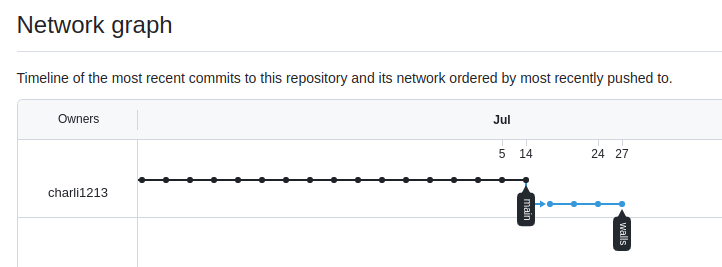
\includegraphics[width=.9\linewidth]{figures/github/Screenshot from 2023-07-28 12-06-35.png}
\label{org728e757}
\end{center}
\end{document}
